\documentclass{article}
\usepackage{caption}
\usepackage{amssymb}
%\usepackage{array}
\usepackage{geometry}
%\usepackage{scrextend}
\usepackage{amsmath}
%\usepackage{hyperref}
\usepackage{graphicx}
\usepackage{pdfpages}
%\usepackage{multicol}
\usepackage{tabularx}
\usepackage{float}

\title{EE102 Homework 2}
\author{Jacob Guenther}

\geometry{
	a4paper,
	total={170mm,257mm},
	left=20mm,
	top=20mm,
}

\begin{document}

\includepdf[pages=1,pagecommand={}]{Lab_4_cover.pdf}

\section{Objective}

\section{Equipment}
\begin{itemize}
	\item Arduino Nano
	\item Resistor
	\item Thermistor
	\item LED
	\item Breadboard
	\item Jumpers
\end{itemize}

\section{Setup}
We use a voltage divider as seen in figure (1).

\begin{figure}[H]
	\begin{center}
	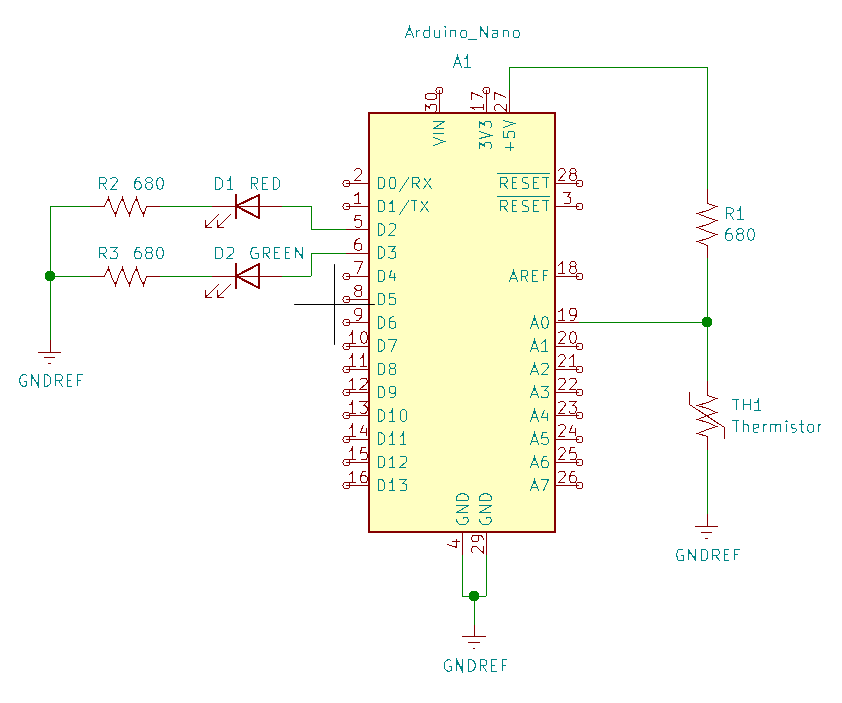
\includegraphics[width=10cm]{schematic}
	\end{center}
	\caption{Voltage divider using the thermistor connected to analog input 0.}
\end{figure}

\section{Observations and Results}

\paragraph{}

\paragraph{}

\begin{figure}[H]
	%\includegraphics[width=10cm]{code}
	\caption{Code used in this lab. Converts analog value to temperature.}
\end{figure}




\newpage
\section{Conclusion}

\newpage
\section{References}
\noindent
[1] Denise Thorsen, Maher Al-Badri, INTRODUCTION TO ELECTRICAL AND COMPUTER ENGINEERING, University of Alaska Fairbanks, 2022.
\newline
\newline
\noindent

\end{document}